\documentclass[11pt,a4paper]{article}
\usepackage[T1]{fontenc}
\usepackage[utf8]{inputenc}
\usepackage{lmodern}
\usepackage{amsmath,amssymb,amsthm,mathtools,mathrsfs}
\usepackage{graphicx,float,xcolor,multicol}
\usepackage[shortlabels]{enumitem}
\usepackage[margin=27mm]{geometry}
\usepackage{microtype,needspace,placeins}
\usepackage{tikz,tikz-cd}
\usetikzlibrary{arrows.meta,calc,positioning,patterns,decorations.pathreplacing}
\usepackage[colorlinks=true,linkcolor=teal,urlcolor=teal,citecolor=teal]{hyperref}
\setlength{\parindent}{0pt}
\setlength{\parskip}{.6em}
\setcounter{secnumdepth}{0}
\allowdisplaybreaks
\raggedbottom
\providecommand{\cross}{\times}
\DeclareUnicodeCharacter{2020}{\ensuremath{\dagger}}
\DeclareMathOperator{\supp}{supp}
\DeclareMathOperator*{\esssup}{ess\,sup}
\providecommand{\chapter}{\section}
\newenvironment{tool}[2]{\subsection*{Tool #1 --- #2}}{}
\newcommand{\ToolRef}[1]{Tool #1}
\newcommand{\FigureTag}[2]{\textit{Figure #1}}
\newcommand{\Result}[1]{\subsection*{#1}}
\newcommand{\Application}[1]{\subsubsection*{Application\if\relax\detokenize{#1}\relax\else\space--- #1\fi}}
\newcommand{\ProofHeading}{\par\textit{Proof.}\space}
\newcommand{\ProofOf}[1]{\par\textit{Proof of #1.}\space}
\newcommand{\RemarkHeading}{\par\textbf{Remark.}\space}
\newcommand{\NoteHeading}{\par\textbf{Note.}\space}
\newcommand{\ExerciseHeading}{\par\textbf{Exercise.}\space}

\graphicspath{{figures/complex-analysis/}}
\begin{document}
\section*{Separation by a Polygonal Path/Arc and Holomorphic Lifting}
% BLOG-CONTENT-BEGIN
\subsection*{Separation by a Polygonal Path/Arc}

Let $U$ be a bounded domain in $\mathbb C$. Then $U$ is simply connected if and only if $\mathbb C\setminus U$ is connected.

First note, very quickly, that a continuous branch of the logarithm on a domain \(U\subset\mathbb C\setminus\{0\}\) is a continuous function \(f:U\to\mathbb C\) such that
\[
  \exp(f(z))=z.
\]
This continuity directly implies holomorphicity, since $\exp'(z)=\exp(z)\ne0$ for every $z\in\mathbb C$. In fact, one has the following. Let $f:U\to V$ be continuous, let $g:V\to\mathbb C$ satisfy $g\in H(V)$ and $g'\ne0$, and suppose $g\circ f\in H(U)$. Then $f\in H(U)$.

\paragraph{Quick proof.} The limit
\[
  \lim_{w\to w_0}
  \frac{g(f(w))-g(f(w_0))}{w-w_0}
\]
exists. Let $f(w_0)=z_0$ and let $f(w_0+h')=z_0+h$. Then
\begin{align*}
  \lim_{h'\to0}
  \frac{g(f(w_0+h'))-g(f(w_0))}{h'}
  &=\lim_{h'\to0}
  \frac{g(f(w_0+h'))-g(f(w_0))}{f(w_0+h')-f(w_0)}\\
  &\qquad\cdot
  \frac{f(w_0+h')-f(w_0)}{h'}.
\end{align*}
The first limit exists and equals some $c$. Consequently,

\[
  \lim_{h'\to0}
  \frac{f(w_0+h')-f(w_0)}{h'}
  =\frac{c}{g'(z_0)}
\]
exists, since $g'\ne0$. Thus $f\in H(U)$, so a continuous branch is a holomorphic branch.


\subsection*{Claim}

There exists a continuous branch of the logarithm $(f,U)$ if and only if $0$ and $\infty$ lie in the same connected component of
\[
  (\mathbb C\cup\{\infty\})\setminus U.
\]

The existence of a continuous branch on $U$ certainly implies that $0$ and $\infty$ are not separated by $U$, since $1/z$ has a primitive---it is conservative in $U$---because any simple closed curve in $U$ cannot contain $0$ in its interior.

For the converse, apply the same construction on the Riemann sphere, using the corresponding form of the Jordan Curve Theorem. Instead of the segments $\overline{xz_0}$, take longitudes joining the North and South poles, $0$ and $\infty$, and then project them back to $\mathbb C$.

\subsection*{Counting the Number of Crossings (Parity Argument)}

Let
\[
  \gamma:[0,+\infty)\to\mathbb C
\]
be a continuous injective map with $\gamma(0)=0$ and
\[
  \lim_{t\to\infty}\gamma(t)=\infty.
\]
Then
\[
  \mathbb C\setminus\gamma([0,+\infty))
\]
is nonempty and simply connected. The image $\gamma([0,+\infty))$ is a branch cut: removing it produces a nonempty simply connected domain on which a single-valued logarithm can be defined.


Since $\lim_{t\to\infty}\gamma(t)=\infty$, we have $|\gamma(t)|>M$ whenever $t>b$. Consider $\gamma([a,b])$, and let $\gamma(b)=z_1$. Choose coordinates so that $\gamma(b)=i$; this can be ensured by an appropriate rotation and dilation. Let $c\in(a,b)$ be such that
\[
  \operatorname{Re}(\gamma(c))=1,
  \qquad
  \operatorname{Im}(\gamma(c))=0.
\]
By simplicity, if
\[
  \gamma_1=\left.\gamma\right|_{[a,c]},
  \qquad
  \gamma_2=\left.\gamma\right|_{[c,b]},
\]
then compactness gives a number $\delta'$, with $0<\delta'<1/10$, such that \(|\gamma_1(t_1)-\gamma_2(t_2)|\ge\delta'\)
whenever
\[
  |\operatorname{Re}(\gamma_1(t_1))|,
  |\operatorname{Re}(\gamma_2(t_2))|\le\frac12.
\]

Let $\gamma^{(N)}$ be a polygonal path approximating
\[
  \gamma:[a,b]\to\mathbb C
\]
such that
\[
  |\gamma^{(N)}(t)-\gamma(t)|<\frac1N.
\]
Let $\{x_i^{(N)}\}_i$ be the crossings of $\gamma^{(N)}$ on the imaginary line segment $\overline{0i}$. We can choose $\gamma^{(N)}$ so that none of its self-crossings or edges lie on $\overline{0i}$. There exists $j$ such that
\[
  x_j^{(N)}\in\gamma^{(N)}([a,c]),
  \qquad
  x_{j+1}^{(N)}\in\gamma^{(N)}([c,b]).
\]
We know that
\[
  \operatorname{dist}\bigl(x_j^{(N)},\gamma([a,c])\bigr)\le\frac1N,
  \qquad
  \operatorname{dist}\bigl(x_{j+1}^{(N)},\gamma([c,b])\bigr)\le\frac1N,
\]
and also
\[
  \operatorname{dist}\bigl(x,\gamma([a,c])\bigr)
  +\operatorname{dist}\bigl(x,\gamma([c,b])\bigr)
  \ge\delta'
\]
for any $x\in[x_j^{(N)},x_{j+1}^{(N)}]$, because of the separation. By the intermediate value property, there exists
\[
  x_*^{(N)}\in(x_j^{(N)},x_{j+1}^{(N)})
\]
such that
\[
  \frac{\delta'}2
  \le\operatorname{dist}\bigl(x_*^{(N)},\gamma([a,c])\bigr)
  =\operatorname{dist}\bigl(x_*^{(N)},\gamma([c,b])\bigr).
\]
Therefore
\[
  \operatorname{dist}\bigl(x_*^{(N)},\gamma([a,b])\bigr)
  \ge\frac{\delta'}2,
\]
and $x_*^{(N)}\notin\gamma([a,b])$. Since $|\gamma(t)|>M$ for $t>b$, and here this is normalized to $1$, we have by continuity $|\gamma(b)|=M$, which here was transformed to $i$. Hence
\[
  x_*^{(N)}\notin\gamma((b,\infty)),
\]
so
\[
  \mathbb C\setminus\gamma([0,+\infty))\ne\varnothing.
\]
To prove that it is simply connected, take any simple closed curve in $\mathbb C$ and note that the interior of that curve cannot meet $\gamma([0,\infty))$; otherwise, as $\gamma$ runs to infinity, it would have to cross the curve. Thus all simple closed curves in $\gamma([0,\infty))^c$ are contractible, so $\gamma([0,\infty))^c$ is simply connected.

\textbf{Remark.} The crucial facts that we exploited are the injectivity of $\gamma$ and the fact that it does not turn back eventually; that is, $\gamma(t)\to\infty$ as $t\to\infty$. The idea is to break the image of $\gamma$ into two compact sets and look at their approximations on a segment. The chosen polygonal approximations meet the transverse segment in finitely many points; hence we can find points that are distant from the broken pieces by looking at their approximations. The Bolzano--Weierstrass theorem then completes the proof.

\subsection*{Holomorphic Lifting}

One way to construct a logarithm is by looking at appropriate domains where $1/z$ can have a primitive, once we make sure it is conservative. There is yet another slick way to do that, via the construction of holomorphic lifts, exploiting concepts in covering-space theory.

\subsection*{Definition: Covering Spaces and Covering Maps}

The map $f:M\to N$ is a covering map if, for every $x\in N$, there exists $U\subseteq N$ such that
\[
  f^{-1}(U)=\bigsqcup_\alpha V_\alpha,
\]
and
\[
  \left.f\right|_{V_\alpha}:V_\alpha\to U
\]
is a homeomorphism.

\begin{figure}[htbp]
  \centering
  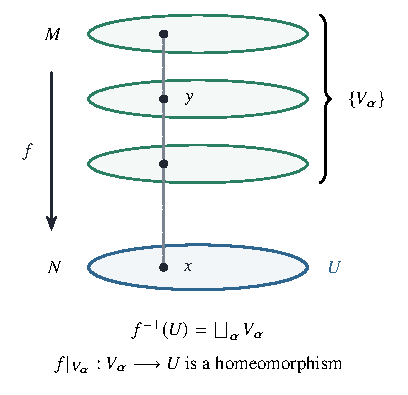
\includegraphics[width=0.62\textwidth]{note8-fig-02.pdf}

\end{figure}


\begin{figure}[htbp]
  \centering
  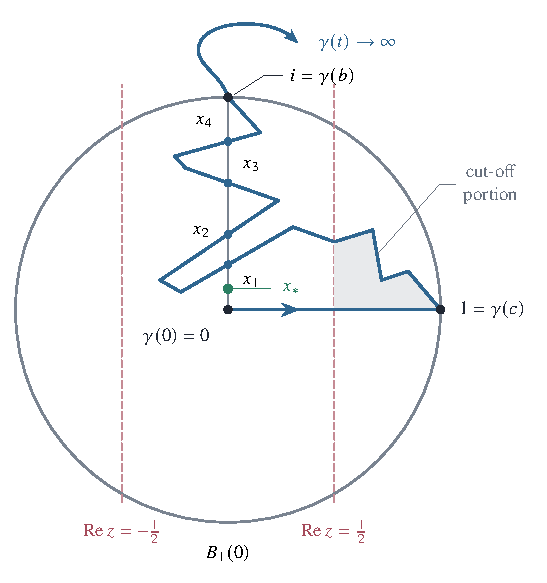
\includegraphics[width=0.72\textwidth]{note8-fig-03.pdf}

\end{figure}

This setup leads to the lifting lemma.

\subsection*{Tool 29 — Lifting Lemma}

Let $M,N$ be Riemann surfaces, let $f:M\to N$ be a covering map, with $M,N$ connected, and let $U$ be a simply connected, path-connected Riemann surface. Let $g:U\to N$ be holomorphic, let $z_0\in U$ and $p\in M$, and suppose \(f(p)=g(z_0).\)
Then there exists a unique holomorphic map $h:U\to M$ such that $h(z_0)=p$ and
\[
  g=f\circ h.
\]


\subsection*{Construction of the Logarithm}

Let \(z:U\to\mathbb C\setminus\{0\},\)
where $U$ is a simply connected domain and $0\notin U$. The map
\[
  e^z:\mathbb C\to\mathbb C\setminus\{0\}
\]
is a covering map. (Exercise.) Hence there exists a holomorphic function $f:U\to\mathbb C$ such that \(\exp(f)=z.\)


More generally, if $h$ is holomorphic and nonvanishing on the simply connected domain $U$, then there exists a holomorphic $g$ such that \(e^{g(z)}=h(z).\)
If we look at
\[
  z^n:\mathbb C\setminus\{0\}\to\mathbb C\setminus\{0\},
\]
which is locally a diffeomorphism, then there exists $g$ such that \(g(z)^n=h(z).\)
% BLOG-CONTENT-END
\end{document}
